%% Template for EU report, using the report.sty style file

\documentclass[12pt,a4paper,twoside]{article}
%% common package
\usepackage[headers]{report}
\usepackage{xspace}
\usepackage{verbatim}
\usepackage[usenames]{color}
\usepackage[usenames,dvipsnames,table]{xcolor}
\usepackage[pdftex,dvips]{graphicx}
\usepackage{url}
\usepackage{array}
\usepackage{color}
%%

%%insert here other packages needed by sections

%%

%%%%%%%%%%%%%%%%%%%%%%%%%%%%%%%%%%%%%%%%%%%%%%%%%%%%%%%%%%%%%%%%%%%%%%%%%%%%%%
%%% Titlepage
%%%%%%%%%%%%%%%%%%%%%%%%%%%%%%%%%%%%%%%%%%%%%%%%%%%%%%%%%%%%%%%%%%%%%%%%%%%%%%

% declaration of variables used in style
\reportDocnumber{Year 1}
\reportTitle{First year periodic report}

\reportAuthor{CoDyCo Consortium}
\reportResponsiblePartner{IIT}
\reportAffiliation{% Insert here authors affiliations
 IIT, TUD, UPMC, UB, JSI.
}

\reportReviewer{}
\reportCoordinator{Francesco Nori}
\reportActivityNumber{1} %% n=1,..,10
\reportActivity{RTD}
\reportDoctype{Periodic report} %% or Prototype
\reportClassification{Public} % or Consortium
\reportDistribution{Consortium} %
\reportStatus{Draft} % Draft or Final
\reportDeliveryDate{28/04/2014}
\reportVersion{1.0}
\reportDate{Apr.~28, 2014}
\reportYear{2014}
\reportPages{\pageref{LastPage}}
\reportChangelog{v.1.0 & Feb 13, 2013 & First draft %%\\\hline
%%              v.2.0 & Feb 20, 2007 & Final version
}
\reportProjectStartingDate{1st March 2013}
\reportProjectEndDate{28th February 2017}
\reportProjectAcronym{CoDyCo}
\reportProjectTitle{Whole-Body Compliant Dynamical Contacts in Cognitive Humanoids}
 \reportContractNumber{600716}
 \reportProjectCoordinator{Istituto Italiano di Tecnologia}
 \reportProjectUrl{www.codyco.eu}
 \reportFrameworkProgramme{FP7}
 
 \reportWorkpackage{All work packages}
 \reportEditors{Francesco Nori, Vincent Padois, Jan Peters, Jan Babic, Michael Mistry}
 \reportContributors{Entire CoDyCo consortium}
 \reportReviewers{-}
\reportAbstract{The scope of the current report is to present the results ...}
\reportReviewers{reviewers}
\reportKeywordList{kw, list, etc, }

%%%%%%%%%%%%%%%%%%%%%%%%%%%%%%%%%%%%%%%%%%%%%%%%%%%%%%%%%%%%%%%%%%%%%%%%%%%%%%
%%% Sections
%%%%%%%%%%%%%%%%%%%%%%%%%%%%%%%%%%%%%%%%%%%%%%%%%%%%%%%%%%%%%%%%%%%%%%%%%%%%%%

%% constants{}

%%%%%%%%%%%%%%%%%%%%%%%%%%%%%%%%%%%%%%%%%%%%%%%%%%%%%%%%%%%%%%%%%%%%%%%%%%%%%%
%%% Misc. by Vincent
%%%%%%%%%%%%%%%%%%%%%%%%%%%%%%%%%%%%%%%%%%%%%%%%%%%%%%%%%%%%%%%%%%%%%%%%%%%%%%
\usepackage{titlesec}
\newcommand{\sectionbreak}{}
\graphicspath{{./images/}}
\usepackage{pdfpages}
\usepackage{caption}
\usepackage{subcaption}
\usepackage{slashbox}
\usepackage{multirow}
\usepackage{appendix}
\usepackage{hyperref}
\hypersetup{
    bookmarks=true,         % show bookmarks bar?
    unicode=false,          % non-Latin characters in Acrobat’s bookmarks
    pdftoolbar=true,        % show Acrobat’s toolbar?
    pdfmenubar=true,        % show Acrobat’s menu?
    pdffitwindow=false,     % window fit to page when opened
    pdfstartview={FitH},    % fits the width of the page to the window
    pdftitle={yearReport.pdf},    % title
    pdfauthor={Vincent Padois},     % author
    pdfsubject={Year 1 report for the CODYCO project},   % subject of the document
    pdfcreator={Vincent Padois},   % creator of the document
    pdfproducer={Vincent Padois}, % producer of the document
    pdfkeywords= {}, % list of keywords
    pdfnewwindow=true,      % links in new window
    colorlinks=true,       % false: boxed links; true: colored links
    linkcolor=black,          % color of internal links (change box color with linkbordercolor)
    citecolor=black,        % color of links to bibliography
    filecolor=black,      % color of file links
    urlcolor=black           % color of external links
}

%%
%%%%%%%%%%%%%%%%%%%%%%%%%%%%%% BEGIN DOCUMENT
\begin{document}

\reportMaketitle


%%TODO move to style
\newcolumntype{L}[1]{>{\raggedright\let\newline\\\arraybackslash\hspace{0pt}}m{#1}}
\newcolumntype{C}[1]{>{\centering\let\newline\\\arraybackslash\hspace{0pt}}m{#1}}
\newcolumntype{R}[1]{>{\raggedleft\let\newline\\\arraybackslash\hspace{0pt}}m{#1}}

\textbf{Document Revision History}
\begin{center}
\begin{tabular}{|C{2cm}|C{3cm}|p{5cm}|C{4cm}|}
\hline
\textbf{Version}&\textbf{Date}&\textbf{Description}&\textbf{Author}\\\hline
First draft & date & description & author\\\hline
\end{tabular}
\end{center}
 
 \clearpage

\newpage
\renewcommand*\contentsname{Table of Contents}
\renewcommand*\listfigurename{Index of Figures}
\tableofcontents
\newpage
\listoffigures
\newpage

%%%%%%%%%%%%%%%%%%%%%%%% Start report content here.

\section{Project objectives for the period}

\subsection{Overview}

\emph{\color{red}[Please provide a short overview of the project objectives for the reporting period in question, as included in Annex I of the Grant Agreement. These objectives are required so that this report is a stand-alone document.]}

\subsubsection{WP1: toolbox for computing and controlling dynamics of whole-body movements with contacts (UB)}

\emph{\color{red}[Please provide a short overview of the work package 1 objectives for the reporting period in question, as included in Annex I of the Grant Agreement. These objectives are required so that this report is a stand-alone document.]}

\subsubsection{WP2: understanding and modelling human whole-body behaviours in physical interaction (JSI)}

\emph{\color{red}[Please provide a short overview of the work package 2 objectives for the reporting period in question, as included in Annex I of the Grant Agreement. These objectives are required so that this report is a stand-alone document.]}

\subsubsection{WP3: control and optimization of whole-body motion in contact (UPMC)}

The objectives of WP3 for the first year of the project are threefold. The first one is to demonstrate the applicability of state of the art whole-body motion controllers, such as the one developed in \cite{salini2012} and \cite{delprete2013}, within the simulation tools evaluated and retained in WP1 and for simple rigid, multi-contact scenarios. The second one is to propose a formulation and a solver for the whole-body control problem at the reactive level that provides a more expressive, richer description of the control problem as well as an efficient way of solving it. The third one is to identify existing or potential ways of optimally coupling the local, reactive control level and the global, decision making one.

\subsubsection{WP4: adaptation, Generalization and Improvement of Compliant Control and Tasks with Contacts (TUD)}

\emph{\color{red}[Please provide a short overview of the work package 4 objectives for the reporting period in question, as included in Annex I of the Grant Agreement. These objectives are required so that this report is a stand-alone document.]}

\subsubsection{WP5: systems integration, standardization and evaluation on the iCub robot (IIT)}

The first year main objective for WP5 was the implementation of a validation scenario consisting of the balancing on different type of rigid contacts. The goal was to include multiple contact positions: feet, hands, back, buttocks, arms and legs. 


\subsubsection{WP6: management (IIT)}

The first year management was primarily dedicated to the project starting. Among the main goals the release of a project software repository.


\subsubsection{WP7: dissemination and Exploitation (IIT)}

The main dissemination objectives for the CoDyCo first year were the creation of a CoDyCo database infrastructure, a CoDyCo project website and participation to dissemination events towards academia and industry. 

\subsection{Follow-up of previous review (if applicable)}

\emph{\color{red}[Please include a summary of the recommendations from the previous reviews (if any) and indicate how these have been taken into account.]}

\section{Work progress and achievements during the period}

\subsection{Progress overview and contribution to the research field}

\emph{\color{red}[Please provide a concise overview of the progress of the work and situate the main achievements in the context of the research field, including a comparative assessment with the current state of the art.]}

\subsubsection{WP1: toolbox for computing and controlling dynamics of whole-body movements with contacts (UB)}

\emph{\color{red}[Please provide a concise overview of the progress of the work and situate the main achievements in the context of the research field, including a comparative assessment with the current state of the art.]}

\subsubsection{WP2: understanding and modelling human whole-body behaviours in physical interaction (JSI)}

\emph{\color{red}[Please provide a concise overview of the progress of the work and situate the main achievements in the context of the research field, including a comparative assessment with the current state of the art.]}

\subsubsection{WP3: control and optimization of whole-body motion in contact (UPMC)}

\emph{\color{red}[Please provide a concise overview of the progress of the work and situate the main achievements in the context of the research field, including a comparative assessment with the current state of the art.]}

After one year of project, the level of achievement of the objectives in WP3 meets the expectations.

The whole-body control frameworks developed by J. Salini and A. Del Prete as part of their respective PhD thesis \cite{salini2012}, \cite{delprete2013} have been tested for simple rigid, multi-contact scenarios in the XDE \cite{XDE} and Gazebo \cite{Gazebo} physics simulators. These two simulators have been retained in WP1 (Deliverable 1.1) as modular simulation frameworks dedicated to the evaluation of the control strategies in CODYCO.

In the meantime, a novel "Generalized Smooth Hierarchical Control" algorithm has been developed \cite{liu2013}. It offers a rich way of describing and solving multi-task problems under constraints: both strict and soft tasks hierarchies can be enforced, tasks can be inserted and removed in a continuous manner and their priorities can be switched smoothly. It appears as a potential alternative to recent work in this domain \cite{escande2012}. Alternatively, TUD has worked on a Bayesian optimization framework dedicated to the bipedal locomotion gait optimization \cite{calandra2014}, \cite{calandra2014b}.

Regarding the exploration of the potential ways of coupling the local, reactive control level and the global, decision making one, several works have been initiated mostly related to the generation of "globally optimal" reference trajectories to be tracked reactively by the local controller. The contributions in this domain over the first year of project are mostly related to the work of A. Ibanez \cite{ibanez2013}, \cite{ibanez2014-icra} and \cite{ibanez2014-ark}. The distributed MPC approach developed in this work tackles the locomotion and balance problem from a new perspective that shares similarities with recent contributions such as \cite{mordatch2012} where an optimization framework enables an automated generation of rich contact behaviors, and \cite{ott2013} that combines a kinesthetic teaching task with an algorithm partially inspired by our approach to improve the balancing behavior during interactions. In the meantime, TUD investigated the interchange of forces during cooperative tasks between humans and robots \cite{berger2013}.

\subsubsection{WP4: adaptation, generalization and improvement of compliant control and tasks with contacts (TUD)}

\emph{\color{red}[Please provide a concise overview of the progress of the work and situate the main achievements in the context of the research field, including a comparative assessment with the current state of the art.]}

\subsubsection{WP5: systems integration, standardization and evaluation on the iCub robot (IIT)}

The first year WP5 activities have concentrated on the first year validation scenario. A complete description of the scenario can be found in ``D5.1 Scientific report on validation scenario 1: balancing on multiple rigid contact points.'' which discusses the technical implementation of the first year validation scenario (see \url{https://github.com/robotology-playground/codyco-deliverables/tree/master/D5.1/pdf}). With respect to the state of the art the work progress represents an implementation of well established torques controlled whole-body control strategies. The integration of tactile feedback within the whole-body controller is a peculiarity of the implemented CoDyCo validation scenario and therefore represent a step forward with respect to the current state of the art. At the moment of writing the current deliverable the iCub tactile sensors cover the feet, the torso, the arms and the hands and the implemented validation scenario accounts for contacts at the hands and feet.

\subsubsection{WP6: management (IIT)}

The CoDyCo project started successfully. Management activities included the definition of an amendment procedure smoothly organized by the consortium and the project officer. A software repository (\url{https://github.com/robotology/codyco}) was set up using state of the art versioning tools (git) and social coding website (\url{https://github.com}). 

\subsubsection{WP7: dissemination and exploitation (IIT)}

Within WP7, CoDyCo first year achievement include: dissemination at relevant academic and industrial events; realization of a CoDyCo experiment database to disseminate robot and humans datasets. 

\subsection{Work package 1 progress}

\subsubsection{Simulator for whole-body motion with contacts (T1.2)}

During year one, UPMC has led several activities related to the simulation of whole-body motion with contacts. These activities are described in deliverable 1.1 and can be summarized as follows:
\begin{itemize}
	\item definition of the requirements for the simulation framework;
	\item survey of the existing simulators for robotics \footnote{http://arxiv.org/abs/1402.7050};
	\item comparison between the XDE and Gazebo iCub simulators and a real iCub performing a free-falling task.
\end{itemize}

\emph{\color{red}[For work package 1 (UB) provide the following information:]}

\begin{itemize}
\item[-] \emph{\color{red}[A summary of progress towards objectives and details for each task;]}
\item[-] \emph{\color{red}[Highlight clearly significant results;]}
\item[-] \emph{\color{red}[If applicable, explain the reasons for deviations from Annex I and their impact on other tasks as well as on available resources and planning;]}
\item[-] \emph{\color{red}[If applicable, explain the reasons for failing to achieve critical objectives and/or not being on schedule and explain the impact on other tasks as well as on available resources and planning (the explanations should be consistent with the declaration by the project coordinator) ;]}
\item[-] \emph{\color{red}[a statement on the use of resources, in particular highlighting and explaining deviations between actual and planned  person-months per work package and per beneficiary in Annex 1 (Description of Work);]}
\item[-] \emph{\color{red}[If applicable, propose corrective actions.]}
\end{itemize}

\subsection{Work package 2 progress}

\emph{\color{red}[For work package 2 (JSI) provide the following information:]}

\begin{itemize}
\item[-] \emph{\color{red}[A summary of progress towards objectives and details for each task;]}
\item[-] \emph{\color{red}[Highlight clearly significant results;]}
\item[-] \emph{\color{red}[If applicable, explain the reasons for deviations from Annex I and their impact on other tasks as well as on available resources and planning;]}
\item[-] \emph{\color{red}[If applicable, explain the reasons for failing to achieve critical objectives and/or not being on schedule and explain the impact on other tasks as well as on available resources and planning (the explanations should be consistent with the declaration by the project coordinator) ;]}
\item[-] \emph{\color{red}[a statement on the use of resources, in particular highlighting and explaining deviations between actual and planned  person-months per work package and per beneficiary in Annex 1 (Description of Work);]}
\item[-] \emph{\color{red}[If applicable, propose corrective actions.]}
\end{itemize}

\subsection{Work package 3 progress}

The progress for each task are described hereafter.

\subsubsection{Reproducing existing control results in a simple case (T3.1)}
During year one, UPMC has achieved task T3.1 by creating a stand-alone C++ library encapsulating the whole-body controller developed in \cite{salini2012} so that it can be used by all partners in simulation or on (any) real humanoid robot. This version of the controller has been tested in rigid multi-contact scenarios in simulation (see Fig.~\ref{fig:xde}) and is currently adapted for tests on the iCub robot.

\begin{figure*}[!ht]
\begin{center}
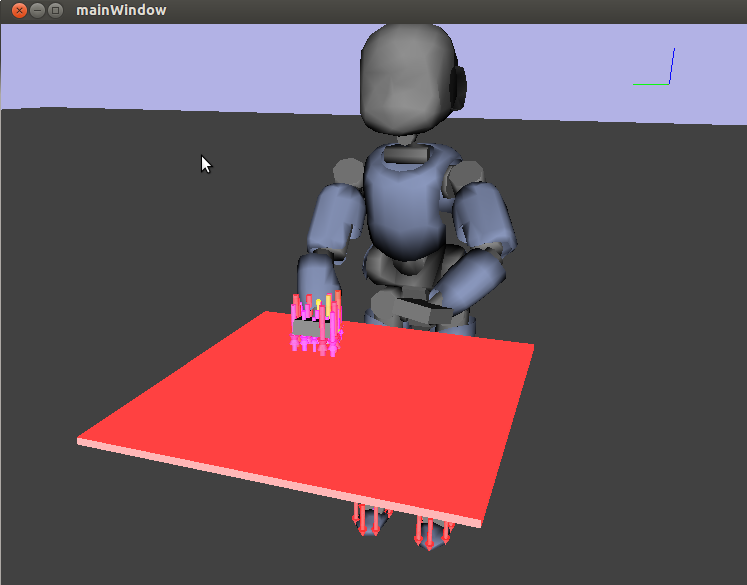
\includegraphics[width=0.3\hsize]{images/s5.png}
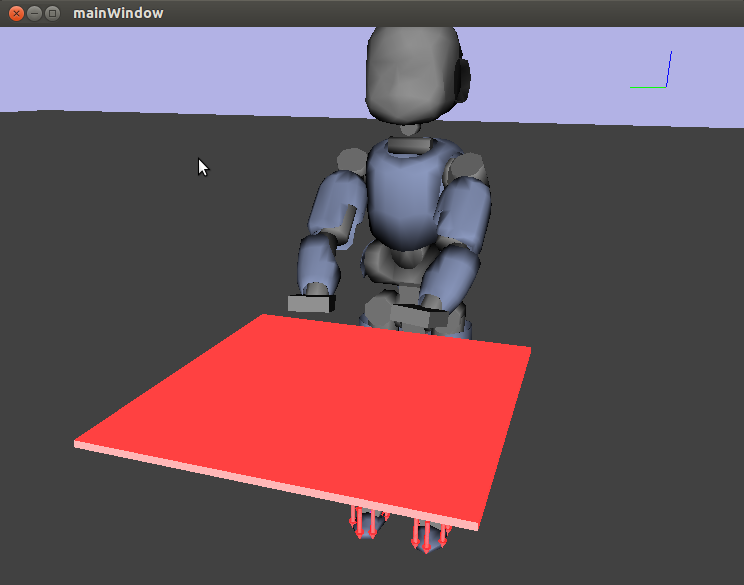
\includegraphics[width=0.3\hsize]{images/s6.png}
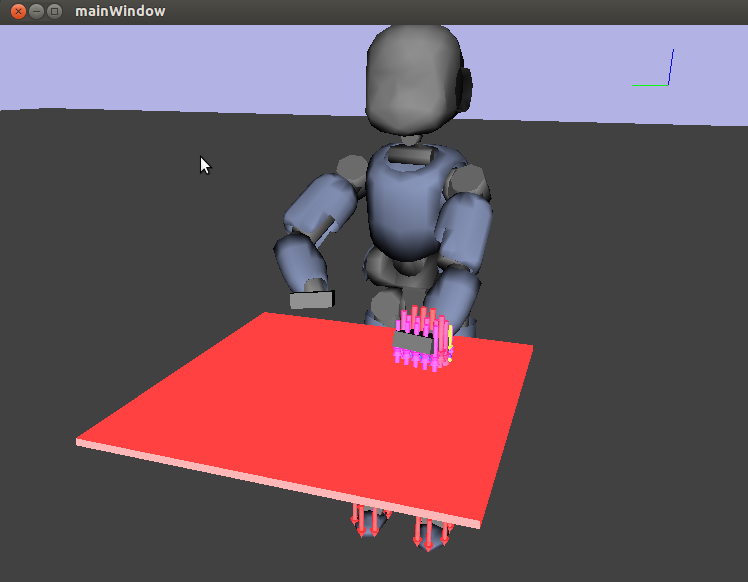
\includegraphics[width=0.3\hsize]{images/s4.png}

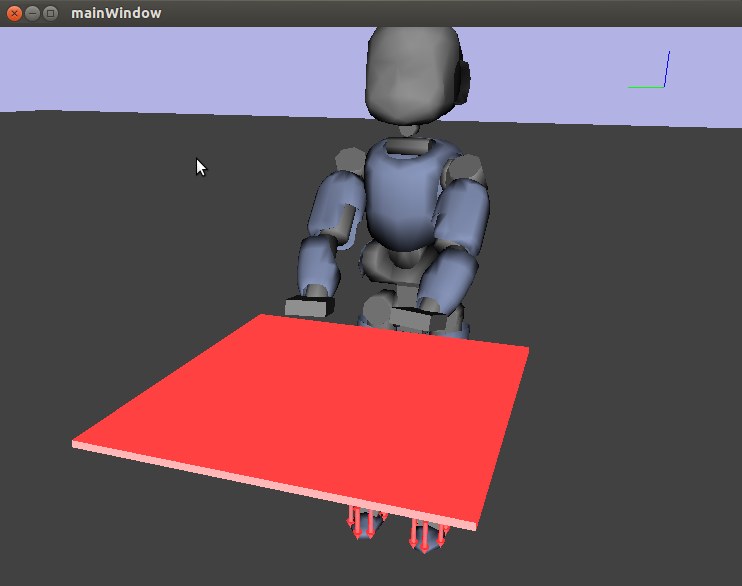
\includegraphics[width=0.3\hsize]{images/s3.png}
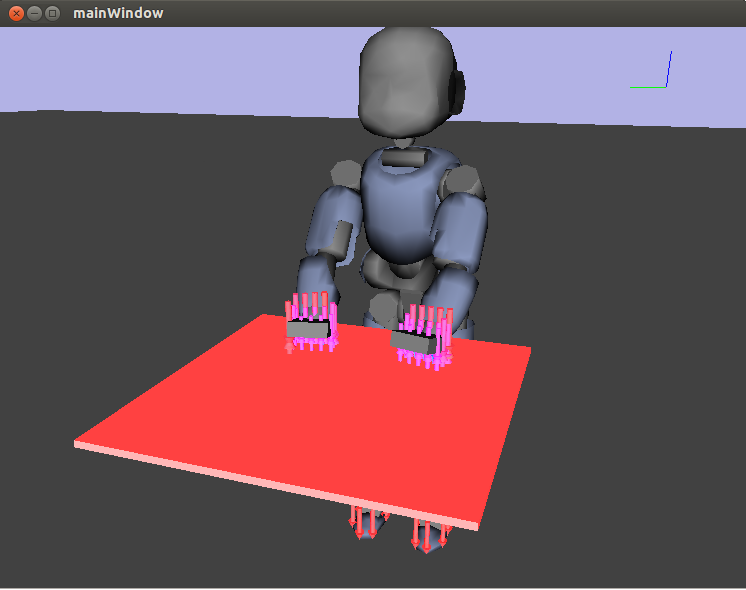
\includegraphics[width=0.3\hsize]{images/s2.png}
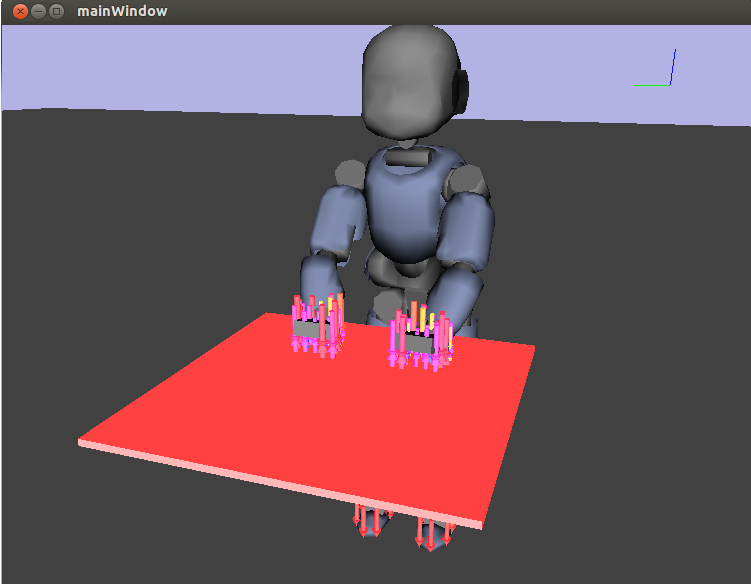
\includegraphics[width=0.3\hsize]{images/s1.png}
\end{center}
\caption{Screenshots of the validation scenario simulated in XDE.}
\label{fig:xde}
\end{figure*}

\subsubsection{Formulating the control problem (T3.2)}

The work performed during year one by UPMC to achieve T3.2 has led to the definition of what a task can be considered to be in the context of the reactive formulation of a multi-task whole body control problem. Among the different characteristics of a task (physical frame, task variable, forward model, desired target trajectory, local controller, priority), the notion of task priority has been largely modified with respect to the classical lexicographic task ordering met in the robotics literature and which is particularly appropriate for cascade resolution approaches such as the one recently proposed in \cite{escande2012}. A partial order has been defined such that task priorities can be described for any pair of task $i$ and $j$. This leads to a richer formulation which includes the original one but is also particularly appropriate for describing task insertion and removal processes as well as priority switching between tasks. Further more, this new prioritization paradigm provides a unique way of defining strict and soft hierarchies between tasks. Associated to this work, the notion  of generalized task projector has been introduced. Each task is associated to a projector which is built based on the tasks priorities. The interest of this projector is that it filters the joint space motion associated to a task so that all priorities are respected, being them soft or strict. Details regarding this work are provided in \cite{liu2013}.

Within this task also IIT contributed with the definition of a software abstraction layer, named wholeBodyInterface (\url{http://wiki.icub.org/codyco/dox/html/namespacewbi.html}). This software library defines the interface to access and control the robot  whole-body. Therefore the wholeBodyLibrary structures the control problem and their definition. Currently the library has been been implemented for both the iCub and the Gazebo iCub simulator.  

\subsubsection{Solving the local control problem (T3.3)}

Associated to the new task formulation proposed in T3.2, the control problem has been formulated by UPMC as an LQP which can be solved by any convex optimization solver dealing with linear constraints. Despite the task hierarchy, the introduction of a generalized task projector per task allows to solve only one LQP. This can be done by introducing as many virtual joint space variables as the number of tasks and using the generalized projector of each task in the expression of the constraints. The resulting problem can be solved by standard convex optimization tools and the cost of introducing virtual joint space variables is compensated for by the fact that only one optimization problem has to be solved. Details regarding this work are provided in \cite{liu2013}.

In the meantime, TUD has proposed to explore optimization methods for solving local control problems that do not require the explicit inversion of any model of the system.  During year one, TUD investigated Bayesian optimization methods that were applied to bipedal locomotion tasks.  One of the key challenges in robotic bipedal locomotion is finding gait parameters that optimize a desired performance criterion, such as speed, robustness or energy efficiency. Typically, gait optimization requires extensive robot experiments and specific expert knowledge. During year one, TUD demonstrated that  data-driven machine learning methods based on Bayesian optimization can be used to automate and speed up the process of gait optimization. These Bayesian optimization methods were used to efficiently find gait parameters that optimize the desired performance metric on a real bipedal walker \cite{calandra2014} and \cite{calandra2014b}.
    

\subsubsection{Bootstrapping and validating the control approach in rigid world and compliant cases (T3.4)}

During year one, UPMC has explored the contribution of MPC approaches to handle the postural balancing problem under varying contact conditions. The hybrid nature of the problem, where varying contact conditions can be accommodated either by adapting the internal forces distribution given a set of contact or by modifying the set of contacts itself, requires control approaches where the desired task trajectories performed through the local, reactive, whole-body controller have to be optimally planned ahead of time in order to provide robust behaviors. The contributions in this domain are mostly related to the work of A. Ibanez \cite{ibanez2013}, \cite{ibanez2014-icra} and \cite{ibanez2014-ark}. The originality of theses contributions lies in:
\begin{itemize}
	\item an augmented ZMP model including external forces exerted directly on indirectly on the center of mass;
	\item a distributed optimization approach that provides a way of generating reference trajectories for the center of mass representing a good compromise given some antagonistic balance and task;
	\item a non scripted foot step placement optimization.
\end{itemize}

UPMC also partially contributed with an experimental study about human behavior during physical contact with the robot. The protocol was registered and obtained the approval of the ethics committee CERES (Conseil d’\'evaluation \'ethique pour les recherches en sant\'e), from University Paris-Decartes. \footnote{Ivaldi et al., "Engagement during human-humanoid interaction", IRB N. 20135200001072.}
The purpose of the experiments is to collect a database of behaviors of experts and naive people interacting physically with the iCub to accomplish a cooperative task. The collected data also include locations of contacts (retrieved through the tactile skin), applied force, robot mouvements: they will be used to study adaptation to human intention during human-robot physical contacts.
    
In the meantime, TUD investigated the interchange of forces during cooperative tasks between humans and robots \cite{berger2013}. Three example scenarios are illustrated in Figure \ref{fig:interaction_tasks}. In such tasks, typically an exchange of forces takes place whenever the interacting agents make contact. Sometimes, forces are even exchanged through an object that is manipulated by both agents, e.g., through a box that is lifted. For a successful execution of such joint physical activities, a robot needs to accommodate for the external forces exerted by a human. To this end, we developed a machine learning approach for identifying external influences and guidance information from humans. During behavior execution by a robot, predictions from a statistical sensor model are continuously compared with stability parameters derived from current sensor readings. Differences between predicted and measured values exceeding the variance of the statistical model are interpreted as perturbations caused by a human and are used to adapt the robot's behavior.
    
\begin{figure}[!ht]
\centering
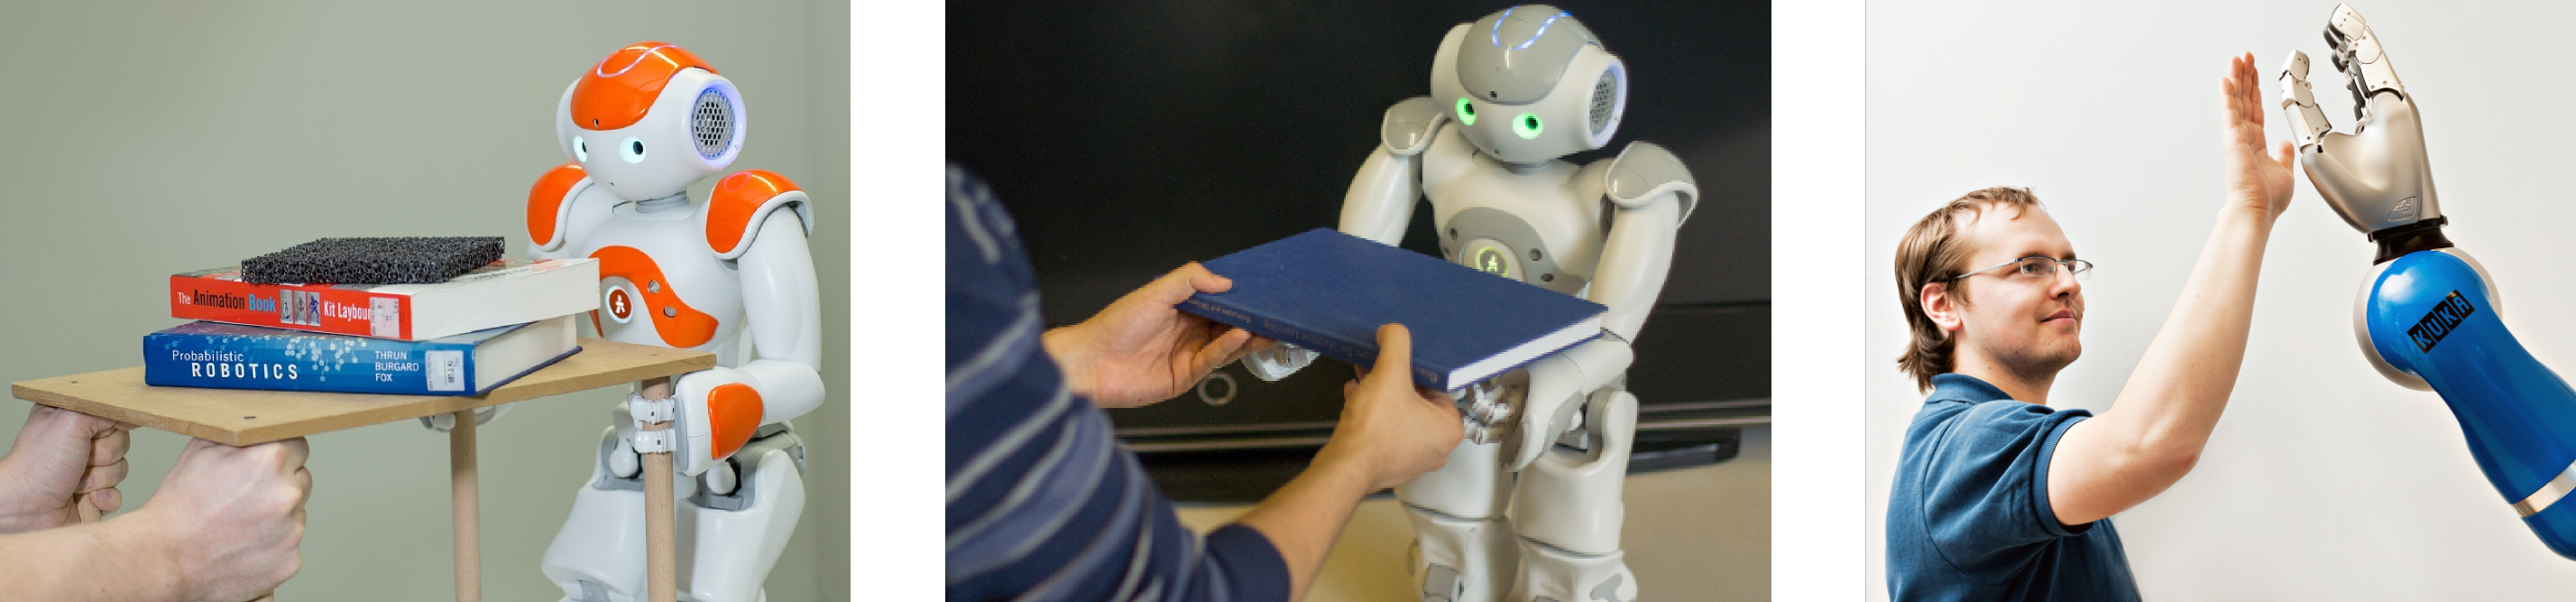
\includegraphics[width=\textwidth]{./pics_tud/interaction_wp3.png}
%\label{fig:subfig2}
 \caption{Illustration of three human robot interaction tasks, where an exchange of forces takes place investigated by TUD during year one.
}
\label{fig:interaction_tasks}
\end{figure}

\subsubsection{Deviations from workplan}  

The PM expenses for WP3 after one year of project are globally conform to the planned one. The observed deviations are related to the fact that tasks 3.3 and 3.4 spans the overall duration of the project and the contribution of some of the partners are expected in the 2nd, 3rd and 4th year.

%\emph{\color{red}[For work package 3 (UPMC) provide the following information:]}
%\begin{itemize}
%\item[-] \emph{\color{red}[A summary of progress towards objectives and details for each task;]}
%\item[-] \emph{\color{red}[Highlight clearly significant results;]}
%\item[-] \emph{\color{red}[If applicable, explain the reasons for deviations from Annex I and their impact on other tasks as well as on available resources and planning;]}
%\item[-] \emph{\color{red}[If applicable, explain the reasons for failing to achieve critical objectives and/or not being on schedule and explain the impact on other tasks as well as on available resources and planning (the explanations should be consistent with the declaration by the project coordinator) ;]}
%\item[-] \emph{\color{red}[a statement on the use of resources, in particular highlighting and explaining deviations between actual and planned  person-months per work package and per beneficiary in Annex 1 (Description of Work);]}
%\item[-] \emph{\color{red}[If applicable, propose corrective actions.]}
%\end{itemize}

\subsubsection{Resources}

\begin{center}
\begin{tabular}{|l|l|l|l|l}
\cline{1-4}
 & Planned PM for year 1 & Actual PM & Comment & \\ \cline{1-4}
IIT & 2 & 2 &  &  \\ \cline{1-4}
TUD & 6 & 4.6 &  &  \\ \cline{1-4}
UPMC & 22.5 & 22 &  &  \\ \cline{1-4}
UB & 2.5 & ? &  &  \\ \cline{1-4}
JSI & 1 & 0 &  &  \\ \cline{1-4}
\end{tabular}
\end{center}

\subsection{Work package 4 progress}

\subsubsection{Generalizing and Improving Elementary Tasks with Contacts (T4.3)}

In the meantime, demonstration-based learning of "optimal trajectories" and stable controllers has been addressed by UPMC, in particular in \cite{stulp2013} where a general, flexible, and compact representation of parameterizable skills is proposed. This work generalizes the standard Dynamic Motor Primitive formulation in \cite{ijspeert2013} and proposes a novel DMP formulation for parametrized skills, based on additionally passing task parameters to the DMP function approximator. This generalizes previous approaches, in particular those which train and execute parametrized skills with two separate regressions. Learning the function approximator with one regression in the full space of phase and tasks parameters allows for more compact models, and the flexible use of different function approximator implementations such as LWPR and GPR, as we demonstrated on the Meka and iCub humanoids robots.


\emph{\color{red}[For work package 4 (TUD) provide the following information:]}

\begin{itemize}
\item[-] \emph{\color{red}[A summary of progress towards objectives and details for each task;]}
\item[-] \emph{\color{red}[Highlight clearly significant results;]}
\item[-] \emph{\color{red}[If applicable, explain the reasons for deviations from Annex I and their impact on other tasks as well as on available resources and planning;]}
\item[-] \emph{\color{red}[If applicable, explain the reasons for failing to achieve critical objectives and/or not being on schedule and explain the impact on other tasks as well as on available resources and planning (the explanations should be consistent with the declaration by the project coordinator) ;]}
\item[-] \emph{\color{red}[a statement on the use of resources, in particular highlighting and explaining deviations between actual and planned  person-months per work package and per beneficiary in Annex 1 (Description of Work);]}
\item[-] \emph{\color{red}[If applicable, propose corrective actions.]}
\end{itemize}

\subsection{Work package 5 progress}

The activities in WP5 are divided into four tasks corresponding to the four years project duration. As a result, during the first year CoDyCo results concentrate on T5.1. The main result consist in the implementation of the validation scenario consisting of the balancing on different type of rigid contacts.

\subsubsection{Scenario 1: iCub balancing on multiple rigid contacts (T5.1)}

The main contributions to T5.1 have been presented in ``D5.1 Scientific report on validation scenario 1: balancing on multiple rigid contact points.'' which discusses the technical implementation of the first year validation scenario (see \url{https://github.com/robotology-playground/codyco-deliverables/tree/master/D5.1/pdf}). The software developed for the scenario implementation is released with an open-source license and distributed through github (\url{https://github.com/robotology/codyco} ). The main software activities include: a module to identify the whole-body motor transfer functions (\url{https://github.com/robotology/codyco/tree/master/src/modules/motorFrictionIdentification}), a module for estimating whole-body internal (joint torques) and external (contact) forces (\url{https://github.com/robotology/codyco/tree/master/src/modules/motorFrictionIdentification}), a module for whole-body joint torque control (\url{https://github.com/robotology/codyco/tree/master/src/modules/jointTorqueControl}), a C++ library that implements the wholeBodyInterface in simulink (\url{https://github.com/robotology/codyco/tree/master/src/simulink}).

\subsubsection{Deviations from workplan}  

The original work plan have foreseen contacts at feet, hands, back, buttocks, arms and legs. The final validation scenario will only include possible contacts at hands and feet. This simplification is mainly due to the fact that at he end of the CoDyCo first year the iCub does not yet include tactile sensing on the back, legs and buttocks. These sensors will be soon included in the iCub and the CoDyCo software is already designed to include this information. 

%\begin{itemize}
%\item[-] \emph{\color{red}[A summary of progress towards objectives and details for each task;]}
%\item[-] \emph{\color{red}[Highlight clearly significant results;]}
%\item[-] \emph{\color{red}[If applicable, explain the reasons for deviations from Annex I and their impact on other tasks as well as on available resources and planning;]}
%\item[-] \emph{\color{red}[If applicable, explain the reasons for failing to achieve critical objectives and/or not being on schedule and explain the impact on other tasks as well as on available resources and planning (the explanations should be consistent with the declaration by the project coordinator) ;]}
%\item[-] \emph{\color{red}[a statement on the use of resources, in particular highlighting and explaining deviations between actual and planned  person-months per work package and per beneficiary in Annex 1 (Description of Work);]}
%\item[-] \emph{\color{red}[If applicable, propose corrective actions.]}
%\end{itemize}

\subsubsection{Resources}

Resources were used as expected.

\begin{center}
\begin{tabular}{|l|l|l|l|l}
\cline{1-4}
 & Planned PM for year 1 & Actual PM & Comment & \\ \cline{1-4}
IIT & 12 & 12 &  &  \\ \cline{1-4}
UPMC & 1 & ? &  &  \\ \cline{1-4}
\end{tabular}
\end{center}

\subsection{Work package 6 progress}

Activities within work package 6 achieved the expected results both in terms of administrative activities and management activities. As a major result, the software repository was successfully implemented thanks to novel versioning tool (git) and social coding website (\url{https://github.com}).

\subsubsection{Administrative coordination (T6.1)}
Administration was successfully coordinated by Chiara Andreoli at IIT. The major activity concerned an amendment that the CoDyCo consortium asked the main reason being the fact that Serena Ivaldi, initially hired by UPMC was recently hired by TUD. Part of the administrative coordination activities were also conducted during three main meetings: the kick-off meeting (Genoa, April 5th, 2013), the simulators meeting (Paris, June 5th, 2013) and the midyear meeting (Paris, November 21st-22nd, 2013). Details on the meetings can be found in the CoDyCo website (\url{http://www.codyco.eu}).

\subsubsection{Software repository implementation (T6.2)}

A github software repository was set up \url{https://github.com/robotology/codyco} and the contribution from the different developers can be directly checked in the website. Relevant information can be found also in ``D6.1 Website and repository online'' available here: \url{https://github.com/robotology-playground/codyco-deliverables/tree/master/D6.1/pdf}.

\subsubsection{Resources}

Resources were used as follows.

\begin{center}
\begin{tabular}{|l|l|l|l|l}
\cline{1-4}
 & Planned PM for year 1 & Actual PM & Comment & \\ \cline{1-4}
IIT        & ? & ? &  &  \\ \cline{1-4}
TUD    & ? & ? &  &  \\ \cline{1-4}
UPMC & ? & ? &  &  \\ \cline{1-4}
JSI       & ? & ? &  &  \\ \cline{1-4}
UB       & ? & ? &  &  \\ \cline{1-4}
\end{tabular}
\end{center}

%\begin{itemize}
%\item[-] \emph{\color{red}[A summary of progress towards objectives and details for each task;]}
%\item[-] \emph{\color{red}[Highlight clearly significant results;]}
%\item[-] \emph{\color{red}[If applicable, explain the reasons for deviations from Annex I and their impact on other tasks as well as on available resources and planning;]}
%\item[-] \emph{\color{red}[If applicable, explain the reasons for failing to achieve critical objectives and/or not being on schedule and explain the impact on other tasks as well as on available resources and planning (the explanations should be consistent with the declaration by the project coordinator) ;]}
%\item[-] \emph{\color{red}[a statement on the use of resources, in particular highlighting and explaining deviations between actual and planned  person-months per work package and per beneficiary in Annex 1 (Description of Work);]}
%\item[-] \emph{\color{red}[If applicable, propose corrective actions.]}
%\end{itemize}

\subsection{Work package 7 progress}

Dissemination and exploitation activities included the participation to international events addressed to both commercial and academic institutions. A preliminary exploitation plan was delineated and reported in the deliverable D7.1.

\subsubsection{Dissemination activities towards academia, industry, and other users (T7.1)}

Dissemination activities were conducted in three main events: (1) iCub exposition at IROS2014, IEEE International Conference on Robotics and Automation Karlsruhe, May 6 - 10, 2013; (2) iCub exposition at the European Robotics Forum and Innorobo, Lyon 29th March 2013; (3) iCub exposition at the European Robotics Forum, Rovereto 12th-14th of March 2014. The full list of papers published within CoDyCo can be found here: \url{http://codyco.eu/publications-menu}.

\subsubsection{Exploitation plan (T7.2)}

The first year activities on T7.1 and T7.2 are all contained in ``D7.1 Dissemination and exploitation plan'' available here: \url{https://github.com/robotology-playground/codyco-deliverables/tree/master/D7.1/pdf}.

\subsubsection{Management of IPR (T7.3)}

No activities to be reported during the first year on this task in consideration of the fact that the task started at the very end of the first year. As a minor starting activity the consortium circulated a list containing each partner responsible contact person for the IPR management. This list is contained in ``D7.1 Dissemination and exploitation plan'' available here: \url{https://github.com/robotology-playground/codyco-deliverables/tree/master/D7.1/pdf}.

\subsubsection{Dissemination of a database of human motion with contacts (T7.4)}

During the first year of CoDyCo, IIT completed the task of setting up a database for storing both human and robot datasets. The details on the database are reported in ``D7.2 Standard database with support materials'' available here \url{https://github.com/robotology-playground/codyco-deliverables/tree/master/D7.2/pdf}. 

\subsubsection{Resources}

Resources were used as follows.

\begin{center}
\begin{tabular}{|l|l|l|l|l}
\cline{1-4}
 & Planned PM for year 1 & Actual PM & Comment & \\ \cline{1-4}
IIT        & ? & ? &  &  \\ \cline{1-4}
TUD    & ? & ? &  &  \\ \cline{1-4}
UPMC & ? & ? &  &  \\ \cline{1-4}
JSI       & ? & ? &  &  \\ \cline{1-4}
UB       & ? & ? &  &  \\ \cline{1-4}
\end{tabular}
\end{center}

%\begin{itemize}
%\item[-] \emph{\color{red}[A summary of progress towards objectives and details for each task;]}
%\item[-] \emph{\color{red}[Highlight clearly significant results;]}
%\item[-] \emph{\color{red}[If applicable, explain the reasons for deviations from Annex I and their impact on other tasks as well as on available resources and planning;]}
%\item[-] \emph{\color{red}[If applicable, explain the reasons for failing to achieve critical objectives and/or not being on schedule and explain the impact on other tasks as well as on available resources and planning (the explanations should be consistent with the declaration by the project coordinator) ;]}
%\item[-] \emph{\color{red}[a statement on the use of resources, in particular highlighting and explaining deviations between actual and planned  person-months per work package and per beneficiary in Annex 1 (Description of Work);]}
%\item[-] \emph{\color{red}[If applicable, propose corrective actions.]}
%\end{itemize}

\bibliographystyle{IEEEtran}
% \bibliography{IEEEabrv,yearReport_WP3,all-ias-publications}
\bibliography{firstYearReport_WP3}

\end{document}

%%% Local Variables:
%%% mode: latex
%%% TeX-master: t
%%% save-place: t
%%% End:
